% Class def
\documentclass[xcolor=table,serif]{beamer} 
\usepackage[square, sort&compress, numbers, sectionbib]{natbib}
\usepackage[spanish]{babel}
\usepackage[none]{hyphenat}
\usepackage[utf8]{inputenc}
%Para incluir detalles cucas del pdf
% \usepackage[pdftex, pdftitle={GENERACIÓN Y CARACTERIZACIÓN DE VÓRTICES
%   ÓPTICOS MEDIANTE MODULADORES ESPACIALES DE LUZ}, pdfauthor={Santiago
%   Echeverri}, pdfsubject={Optical Vortices, SLM Characterization,
%   Phase retrieval}, pdfkeywords={Optical Vortices, SLM
%   Characterization, Phase retrieval},
% pdfpagemode=UseOutlines,bookmarks,bookmarksopen,pdfstartview=FitH,colorlinks,linkcolor=blue,
% urlcolor=black, cite color=red]{hyperref} %
%\usepackage[hyperpageref]{backref} 
% For text justification
\usepackage{ragged2e}
%\usepackage{animate} %need the animate.sty file 
% ams math packages
\usepackage{amsmath}
\usepackage{amsfonts}
\usepackage{amssymb}
% % Images 
 \usepackage{graphicx}
 \usepackage{subfigure}
 \usepackage[labelformat=empty]{caption}
 \setbeamerfont{caption}{size=\scriptsize}
% theme 
\usetheme[]{Madrid}
\usecolortheme{dolphin}
% Links and hyperlinks
\usepackage{url}
% \usepackage{hyperref}
\hypersetup{colorlinks, linkcolor = blue, urlcolor = blue}
% Default fixed font does not support bold face
\DeclareFixedFont{\ttb}{T1}{txtt}{bx}{n}{8} % for bold
\DeclareFixedFont{\ttm}{T1}{txtt}{m}{n}{8}  % for normal
% For text boxes
\usepackage{fancybox}

\usepackage{listings}
% Python style for highlighting

\date{\today} 
\newif\ifplacelogo % create a new conditional
\placelogotrue % set it to true
\logo{\ifplacelogo Maestría en Física Aplicada\includegraphics[width=1cm]{Figures/presentation/EAFIT.jpg}\fi} 
\author[]{Santiago Echeverri Chac\'on\\ Director: René Restrepo
  Gomez\\Co-director: Luciano A Ángel Toro}
\title[Trabajo de grado]{GENERACIÓN Y CARACTERIZACIÓN DE VÓRTICES
                  ÓPTICOS MEDIANTE MODULADORES ESPACIALES DE LUZ}
\subtitle{Trabajo de grado}
\institute{Universidad EAFIT}

\setbeamertemplate{footline}
{
  \leavevmode%
  \hbox{%
  \begin{beamercolorbox}[wd=.2\paperwidth,ht=2.25ex,dp=1ex,center]{author in head/foot}%
    \usebeamerfont{author in head/foot}Universidad EAFIT
  \end{beamercolorbox}%
  \begin{beamercolorbox}[wd=.8\paperwidth,ht=2.25ex,dp=1ex,right]{title in head/foot}%
    \usebeamerfont{author in head/foot}\insertshorttitle\hspace*{3em}
    \insertsection\hspace*{1em}\insertsubsubsection\hspace*{1em} 
    \insertframenumber{} / \inserttotalframenumber\hspace*{1ex}
  \end{beamercolorbox}}%
  \vskip0pt%
}

\begin{document}

\begin{frame}
\titlepage
\end{frame}
\frame{
\footnotesize 
\frametitle{Contenido}
\tableofcontents
}
\AtBeginSection[]
{
 \begin{frame}
   \frametitle{Contenido}
   \footnotesize 
   \tableofcontents[currentsection]%,hideothersubsections]
   \normalsize
\end{frame}
}

\section{Introducción}
\subsection{Planteamiento del Problema}
\begin{frame}
\frametitle{Planteamiento del problema}
Lograr la manipulación del momento angular de la luz abre campo a una
gran cantidad de aplicaciones en numerosas áreas de la ciencia. 
\end{frame}
\placelogofalse
\frame{
  \frametitle{Applicaciones de haces con VOs}
  \begin{figure}
    \includegraphics[scale = 0.5]{Figures/presentation/terabit_com_application.png}
  \end{figure}
}
\frame{
  \frametitle{Applicaciones de haces con VOs}
  \begin{figure}
    \includegraphics[scale = 0.5]{Figures/presentation/phase_microscopy.png}
  \end{figure}
}
\frame{
  \frametitle{Applicaciones de haces con VOs}
  \begin{figure}
    \includegraphics[scale = 0.45]{Figures/presentation/spiral_interferometry.png}
  \end{figure}
}

\subsection{Contexto}
   \placelogotrue
 \begin{frame}
   \frametitle{Contexto}
   \begin{block}{\centering Proyecto interinstitucional en curso} 
	\justifying
   Aberraciones ópticas en haces Laguerre-Gaussianos:
       corrección y aplicaciones metrológicas; 2013 – 2015
   \end{block}
   \begin{figure}
     \centering
     \includegraphics[scale = .5]{Figures/presentation/instituciones.png}
   \end{figure}
 \end{frame}

 \begin{frame}
   \frametitle{Contexto}
   \begin{figure}
     \centering
     \includegraphics[scale = .5]{Figures/presentation/jovenes_inv_conv.png}
   \end{figure}
 \end{frame}
 \begin{frame}
   \frametitle{Contexto}
   \begin{figure}
     \centering
     \includegraphics[scale = .5]{Figures/presentation/inta_conv.png}
   \end{figure}
 \end{frame}

\subsection{Objetivos}
\begin{frame}
  \frametitle{Objetivos planteados en el anteproyecto}
  \begin{block}{Objetivo General}
    Desarrollar la capacidad para generar y caracterizar vórtices de fase
    mediante un SLM de transmisión. 
  \end{block}
  \begin{block}{Objetivos Espec\'ificos}
    \small
    \begin{enumerate}
	\item Identificar y apropiar los conceptos y
                  procedimientos necesarios para caracterizar
                  moduladores espaciales de luz de transmisión, con
                  miras a la producción y análisis de vórtices
                  ópticos. 
        \item Implementar una plataforma experimental para
                  caracterizar la modulación de amplitud y fase de un
                  SLM a partir de un montaje interferométrico
                  automatizado. 
         \item Obtener experimentalmente vórtices ópticos del
                  tipo Laguerre-Gauss mediante el uso de un SLM y
                  estudiar las distribuciones de intensidad y fase
                  alrededor de los vórtices. 
         \item Proponer alternativas para el desarrollo de
                  aplicaciones metrológicas basadas en la generación
                  de VOs y el estudio de sus propiedades.
       \end{enumerate}
     \end{block}
   \end{frame}
 \subsection{Justificación}
 \begin{frame}
   \frametitle{Justificación}
  \end{frame}

\section{Generación de Vórtices Ópticos}
\subsection{Introducción}
\subsection{Marco Teórico}
\subsection{Caracterización de un SLM de transmisión}
\subsection{Resulatados experimentales}

\section{Caracterización de aberraciones de Vórtices Ópticos}
\subsection{Introducción}
\frame{
  \frametitle{Fuentes de aberraciones}
\begin{columns}[t]
\column{0.5 \textwidth}
Pueden deberse a imperfecciones en:
\begin{itemize}
  \item el diseño,
  \item los materiales,
  \item la manufactura,
 \item o la alineación 
\end{itemize}
de elementos ópticos.
\vspace{0.5cm}

Y en nuestro caso, a los efectos no deseados que introducen algunas
características del SLM como las distintas formas de discretización
y el factor de llenado.
\column{0.5 \textwidth}
\begin{figure}
  \includegraphics[scale = .25]{Figures/presentation/discrete_mask2.png}
\end{figure}
\begin{figure}
\includegraphics[scale =.5]{Figures/presentation/fill_factor.jpg}
\caption{}
\end{figure}
\end{columns}
}
\frame{
\frametitle{¿Cómo caracterizar las aberraciones?}
\begin{figure}
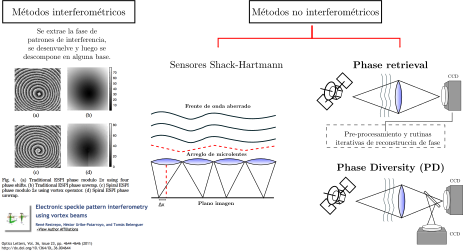
\includegraphics[scale = .9]{Figures/presentation/retrieval_methods.pdf}
\end{figure}
}
\frame{
\frametitle{Phase Diversity tradicional}
Phase Diversity busca frentes de onda que produzcan intensidades en un
plano im'agen que coincidan con las medidas experimentales de la PSF. 
\begin{columns}


\end{columns}
}
\subsection{Marco teórico}
\subsection{Aberraciones simuladas}
\subsection{Aberraciones experimentales}

\section{Conclusiones y trabajo futuro}	
	\begin{frame}{Conclusiones}
	\begin{itemize}
\item Se mostró el resultado de una labor investigativa con la cual
  fue posible establecer un marco conceptual y teórico para la
  caracterización y puesta a punto de un modulador espacial de luz de
  trasmisión basado en cristales líquidos del tipo twisted nematic. 
\item Se presentó un sistema automatizado para la caracterización de
  pantallas de cristál líquido que se compone de una parte física, que
  involucra cuatro rotadores ópticos mecatrónicos, y una parte de
  software que adquiere los datos y los procesa para obtener las
  matrices de Jones que describen el elemento birrefringente para cada
  nivel de gris. 
\item Asimismo, se desarrolló y puso en proceso de registro una aplicacion de software en la
  plataforma Matlab$\circledR$ para la
  generación de máscaras de fase arbitrarias a ser proyectadas en el
  SLM. Esta aplicación permite:
  \begin{itemize}
    \item Crear máscaras de fase espiral de carga entera arbitraria
      sumadas a:
      \begin{itemize}
        \item Lentes.
        \item Rejillas de difracción de varios tipos.
        \item Aberraciones ópticas compuestas a partir de polinomios
          de Zernike.
      \end{itemize}
    \item Discretizar las máscaras de fase en la cantidad de niveles
      deseados, y asignando valores predeterminados a cada uno. 
  \end{itemize}
% \item Por otra parte, se propuso un método novedoso para la
%   caracterización de SLMs basado en el análisis de desplazamiento de
%   franjas en un interferómetro con brazos que no comparten el mismo
%   estado de polarización. Este método ha sido demostrado en
%   simulaciones y nos encontramos en el proceso de corroboración
%   experimental para validarlo. 
 \item Utilizando una configuración de estados de polarización que
   producen alta modulación de fase y baja modulación de amplitud se
   generaron VOs en un sistema óptico 4F usando dos tipos distintos de
   máscaras de fase. Se concluyó que para obtener VOs de calidad es
   prefereible usar máscaras del tipo tenedor sobre máscaras espiral y
   se detectó que aún con buena modulación no se corrigen del todo las aberraciones. 
\item Dado lo anterior se desarrolló un método traído de aplicaciones
  en astronomía para la detección y corrección de aberraciones ópticas en haces con vorticidad óptica.
\item Este método fue validado mediante numerosas simulaciones, y
  experimentos y se propuso como la base para un instrumento que puede
  ser usado en aplicaciones metrológicas. 
\end{itemize}
\end{frame}

\begin{frame}
  \frametitle{Trabajo futuro}
    ¿Qué vale la pena explorar en trabajos futuros?	
\end{frame}
\begin{frame}{¿Preguntas?}
  \begin{figure}
    \centering
    \includegraphics[scale=0.5]{Figures/presentation/thinker.jpeg}	
  \end{figure}
\end{frame}

\section{Bibliograf\'ia}
  \begin{frame}[allowframebreaks]
  \frametitle{Bibliograf\'ia}
  \bibliographystyle{unsrt}
  \bibliography{References/presentation_references}
  \end{frame}
\end{document}
